\documentclass[a4paper,11pt]{article}

\usepackage[T1]{fontenc}
\usepackage[active]{srcltx}
\usepackage[english]{babel}
\usepackage[numbers]{natbib}
\usepackage[utf8]{inputenc}
\usepackage{amsmath}
\usepackage{amssymb}
%\usepackage{fullpage}
\usepackage{graphicx}
\usepackage{listings}
\usepackage{parskip}
\usepackage{srcltx}
\usepackage{url}

\urlstyle{same}

\newcommand{\m}[1]{\boldsymbol{#1}}
\renewcommand{\*}[0]{\cdot}
\renewcommand{\Pr}[1]{\mathbf{Pr}[#1]}
\renewcommand{\v}[1]{\vec{#1}}
\newcommand{\trans}[2][eng.]{(#1 \emph{#2})}

\title{
    {\sc DD2380 Artificial intelligence} \\
    Project report from group PIMP
}
\author{
    Joel Bohman \\ 881117 \and
    Samuel Lidén Borell \\ 881230 \and
    Joel Pettersson \\ 880519 \and
    Linus Wallgren \\ 880213
}
\date{\today}

\begin{document}
\maketitle
\thispagestyle{empty}
\newpage
\begin{abstract}
    % TODO write abstract
\end{abstract}
\thispagestyle{empty}
%\mbox{}
%\thispagestyle{empty}
\newpage
\setcounter{page}{1}

\section{Introduktion}


Test \cite{culberson1997}.

Testing \cite{russell2009}.

Testing \cite{takes2007}.

\begin{figure}[h]
    \begin{center}
        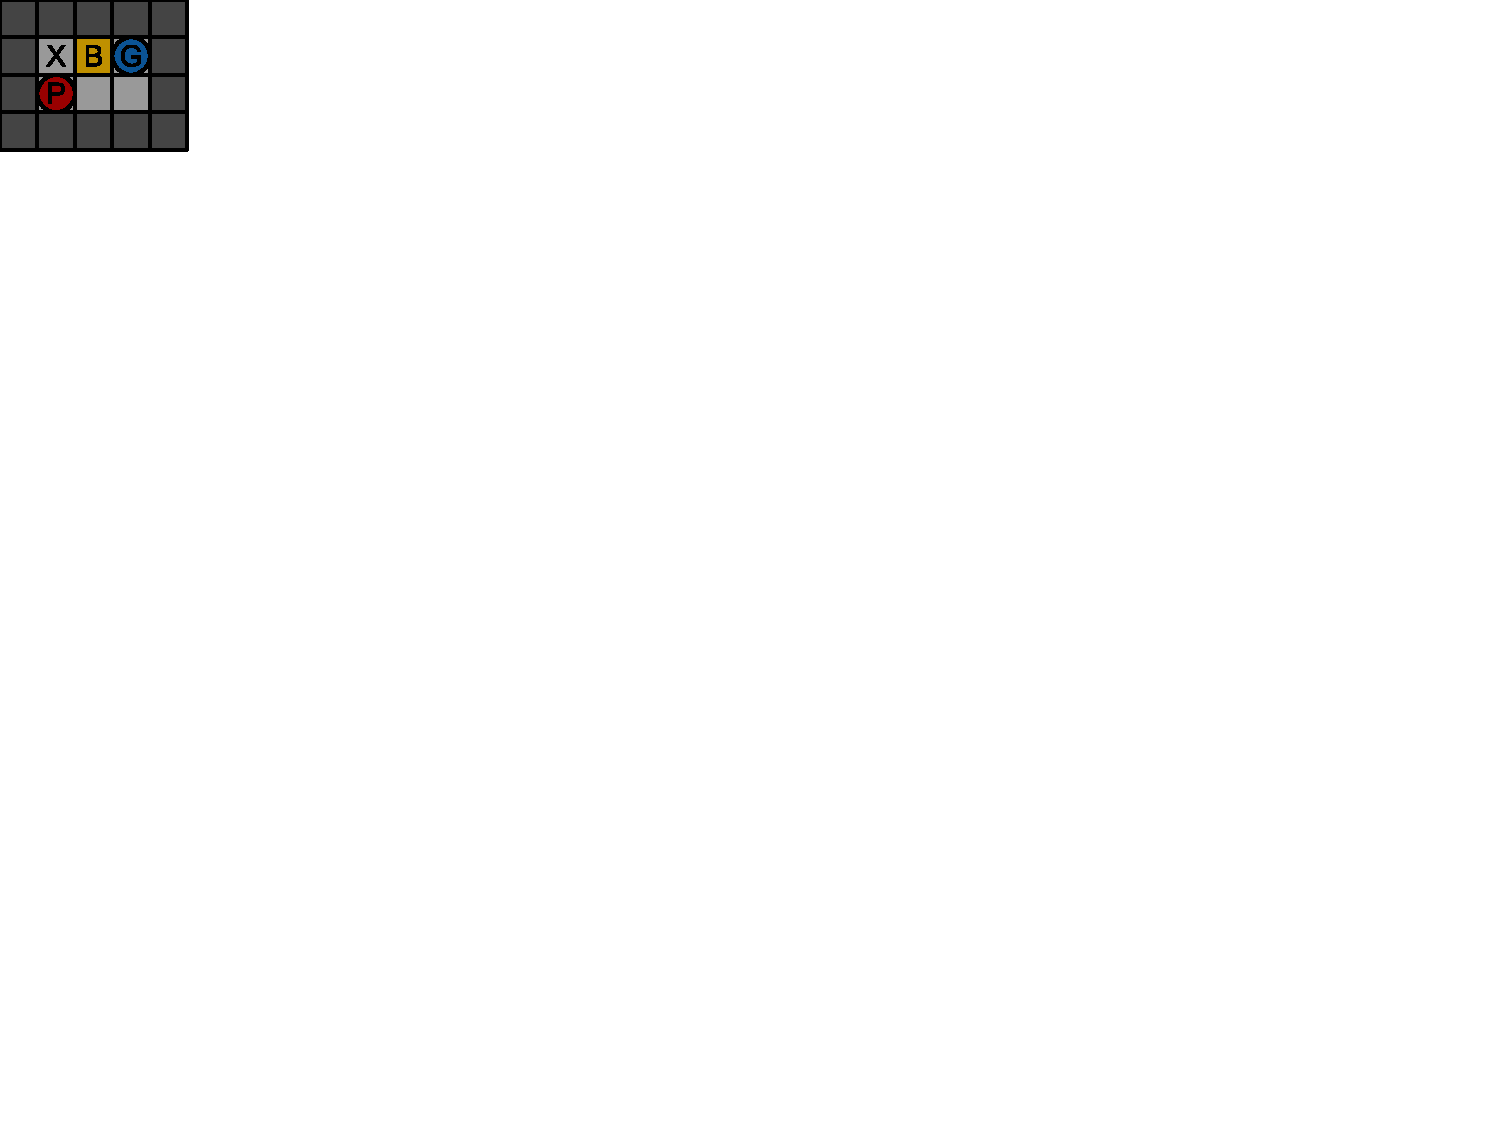
\includegraphics{figures/equalState1}
    \end{center}
    \caption{Test}
    \label{fig:test}
\end{figure}


\bibliographystyle{plainnat}
\bibliography{references} 


\end{document}
